\documentclass{article}
\usepackage{graphicx}
\usepackage{float}

\title{IdentiFisher: \\ User Guide \\}



\author{
\Large McDonald, Christopher\\
\texttt{1312456} \\ \\
\Large Guo, Tian\\
\texttt{1327833} \\ \\
\Large Murray, Shandelle\\
\texttt{1303109} \\ \\
\Large Cheung, Ocean\\
\texttt{1316057} \\
}

\vfill
\date{\today}

\begin{document}
\maketitle

\newpage
\tableofcontents
\vfill
\noindent \\


\pagebreak
\section{Introduction}

\subsection{Purpose of Application}
The purpose of the IdentiFisher application is to identify a fish when caught in a particular area
by searching a database of fish by identifiable properties. These properties are easily distinguished
such as colour, pattern, and shape. This application is designed for beginners who lack the knowledge
to distinguish the fish they have caught.

\subsection{Developers}
The software system IdentiFisher is an Android application.
This system will be a utility application for anyone who fishes, either recreationally or
competivitely. It will service beginner to experienced fishers. Identifisher will allow
the user to give information about a recently caught fish and help to identify what type
of fish it is. From there, it can collect data and track which types of fish are caught where. The aim is to
build a global logging system that will provide percentage catch rates by lake,
educate young, novice fishers, and integrate technology into a relatively non-technological field.


\section{Instruction}
This section will discuss the layout of each page of the application and the respective functions.
Walkthrough of how to complete a task will also be presented.

\subsection{Main Page}
The main page controls the display of other pages and their respective functions. The user may navigate to the
appropriate page from the main page based on what function is needed. \\

\begin{figure}[H]
	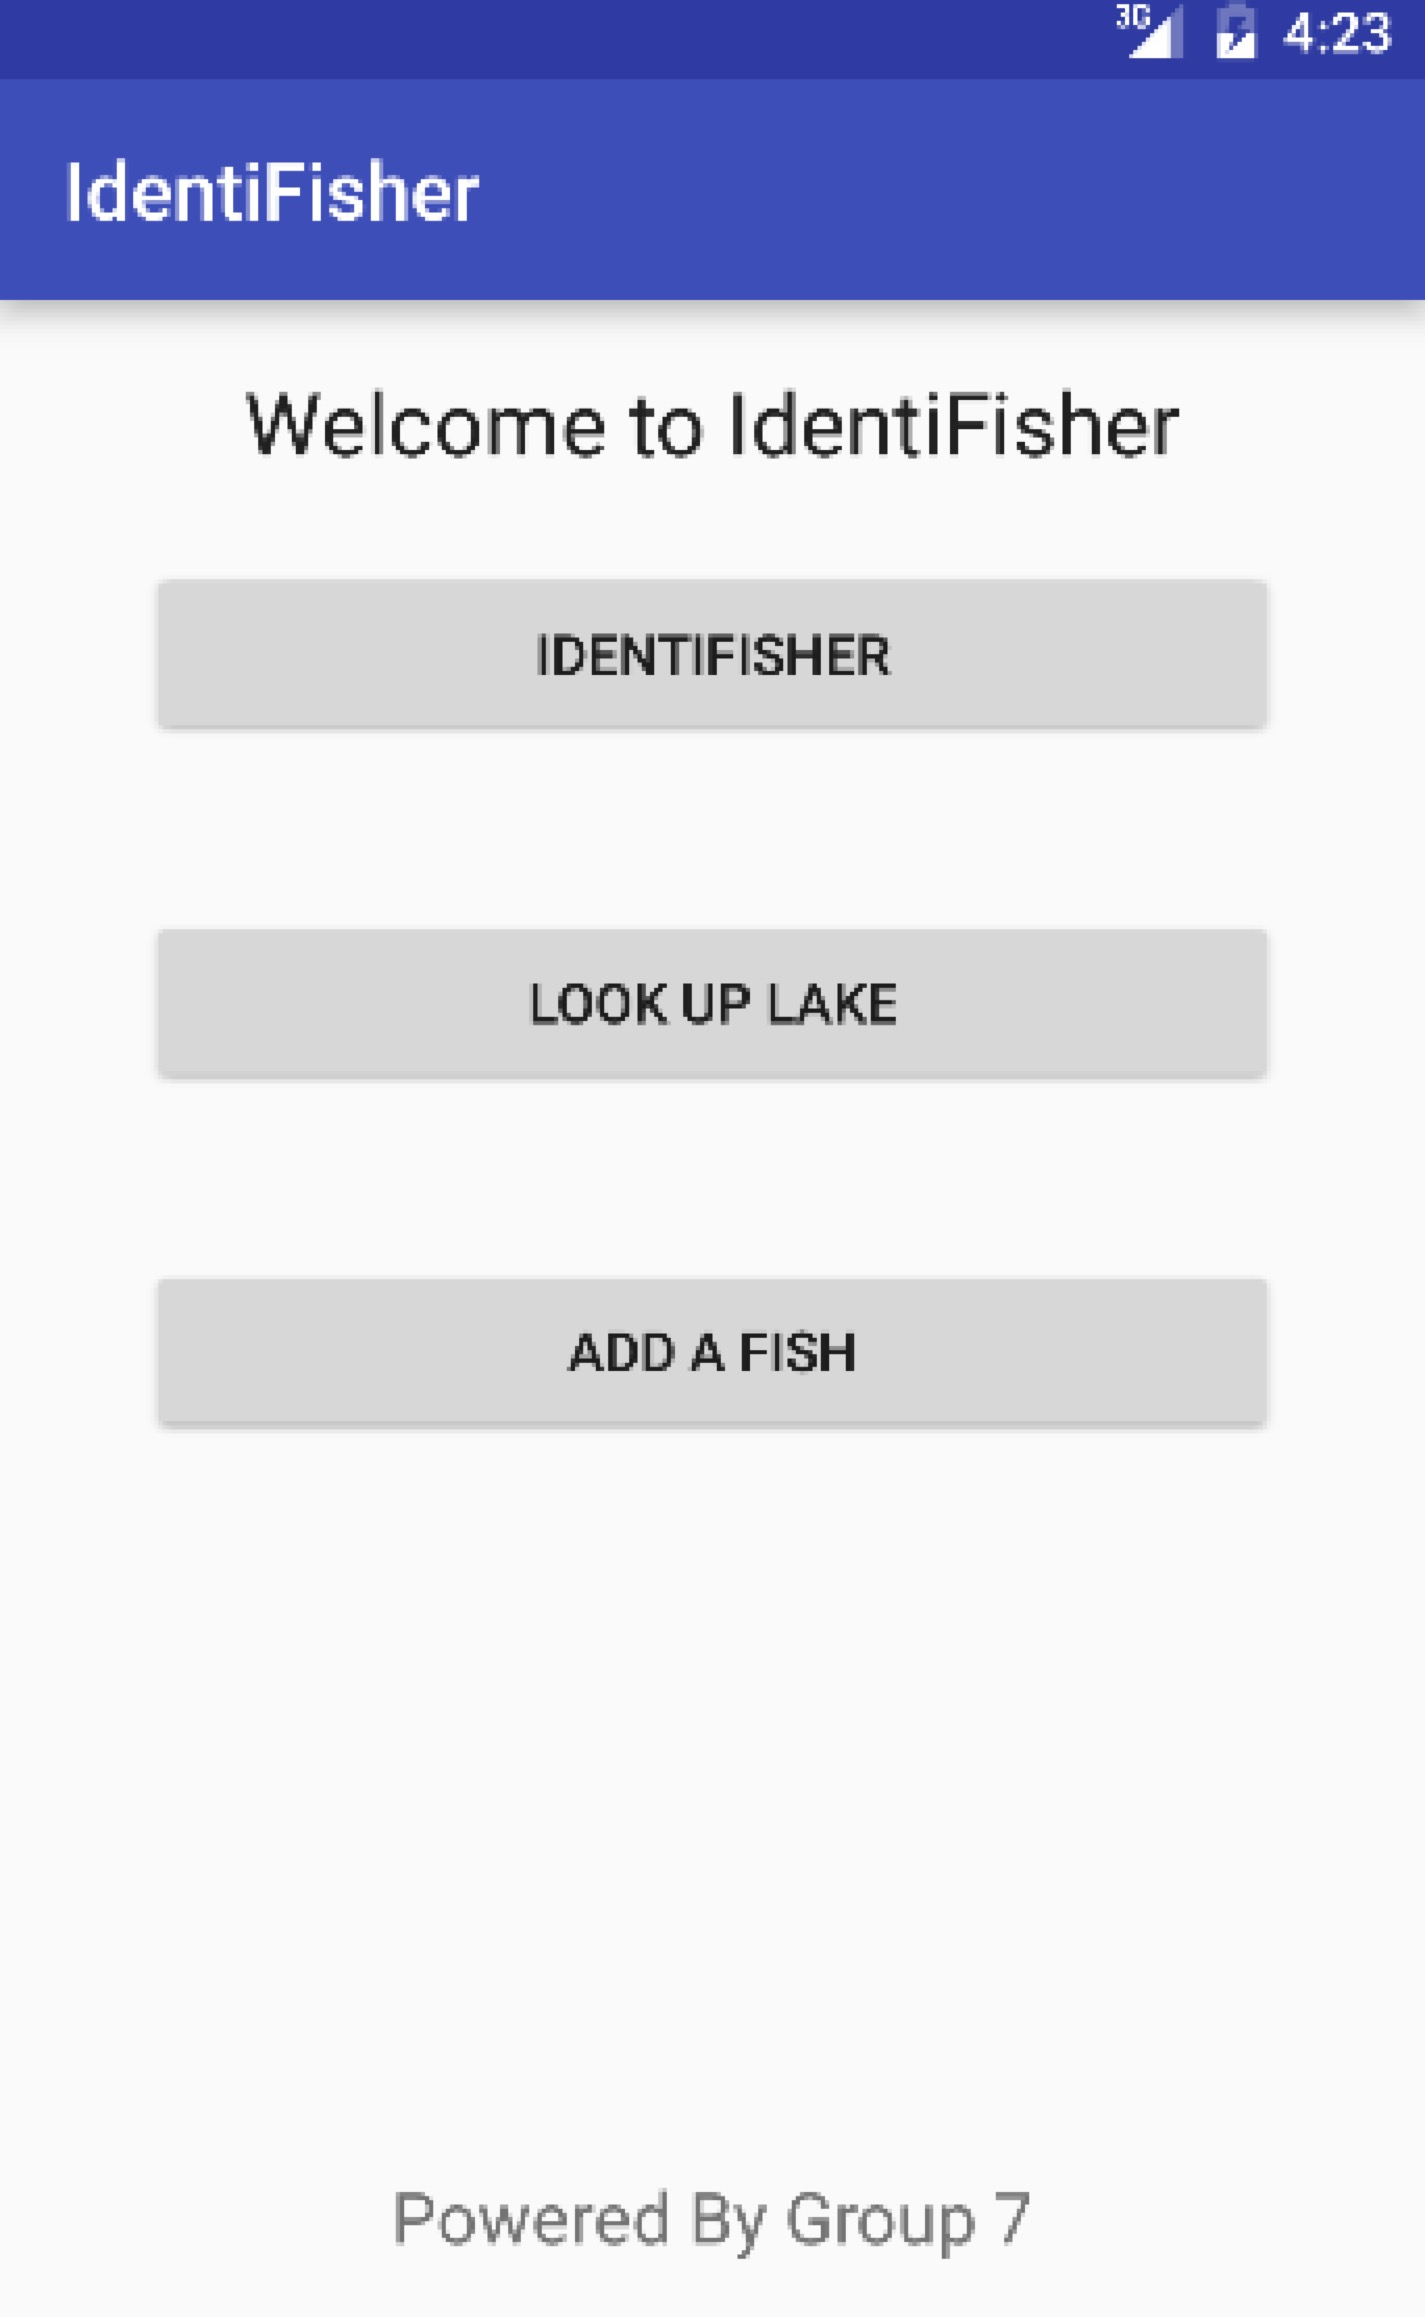
\includegraphics[scale=0.16]{Mainpage.png}
	\caption{Main page of IdentiFisher Application}
\end{figure}

The main page has the name of the application and the welcome message at the top of the screen. There are three
buttons that when pressed will navigate to a different page. The  \textit{IDENTIFISHER} button will take the user to a page
where the user will select different properties of a fish to identify. The \textit{LOOK UP LAKE} button will navigate to a page where the
user may search up a lake near a certain location to find the possible list of fish in the area. The \textit{ADD A FISH} button will navigate
to a page where the user may add a fish with a location of fish found to the database of the app.\\

\subsection{IDENTIFISHER page}
The IDENTIFISHER page displays an instruction message at the top of the page: \textit{Please enter the following criteria}. There are three
drop down menus for colour, pattern, and shape of the fish respectively. There is a "IDENTIFY!" button underneath that the user can
start the identification when the correct properties are selected.\\

\begin{figure}[H]
	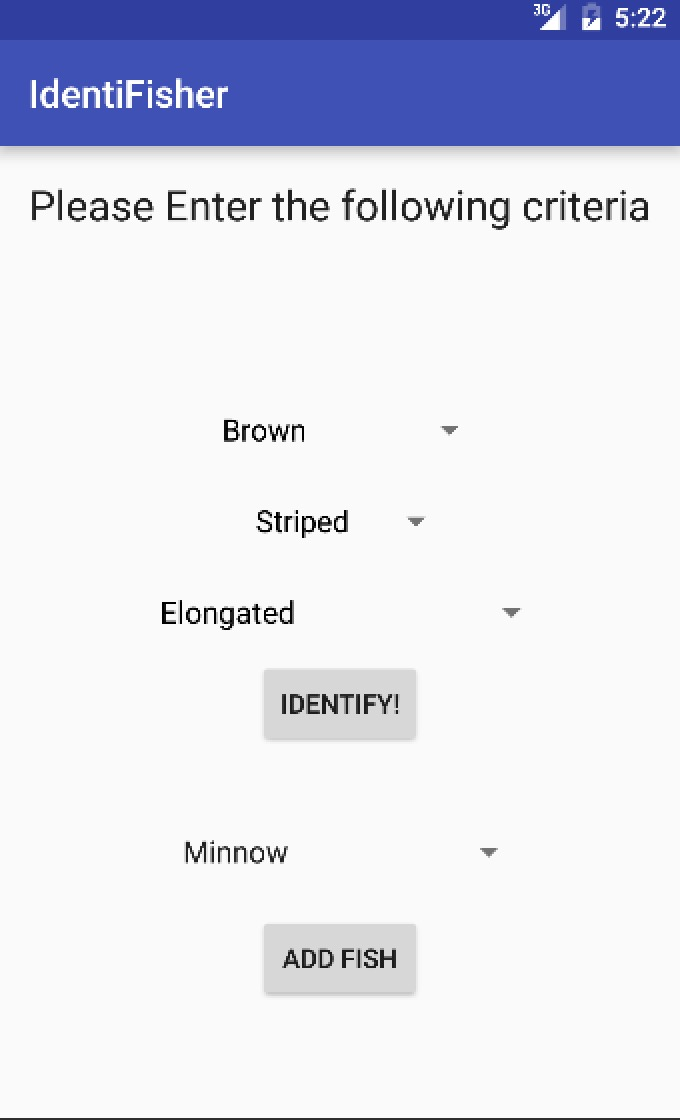
\includegraphics[scale=0.30]{IdentiFisher.png}
	\caption{IDENTIFISHER page of IdentiFisher Application}
\end{figure}

After hitting the "IDENTIFY!" button, the application will display the most likely fish underneath. The user can also click on the drop-down
menu to display a list of other possible species of fish. Finally the user may add the fish to the database by pressing the \textit{ADD FISH} button.\\

\subsection{LOOK UP LAKE page}
The LOOK UP LAKE page has a title of the page and instruction at the top prompting the user to input a location. There is a text field for input and a
\textit{FIND MY LAKE} button. Once pressed with an input in the text field the program will return a database of fish that can be found within the
region\\
\begin{figure}[H]
	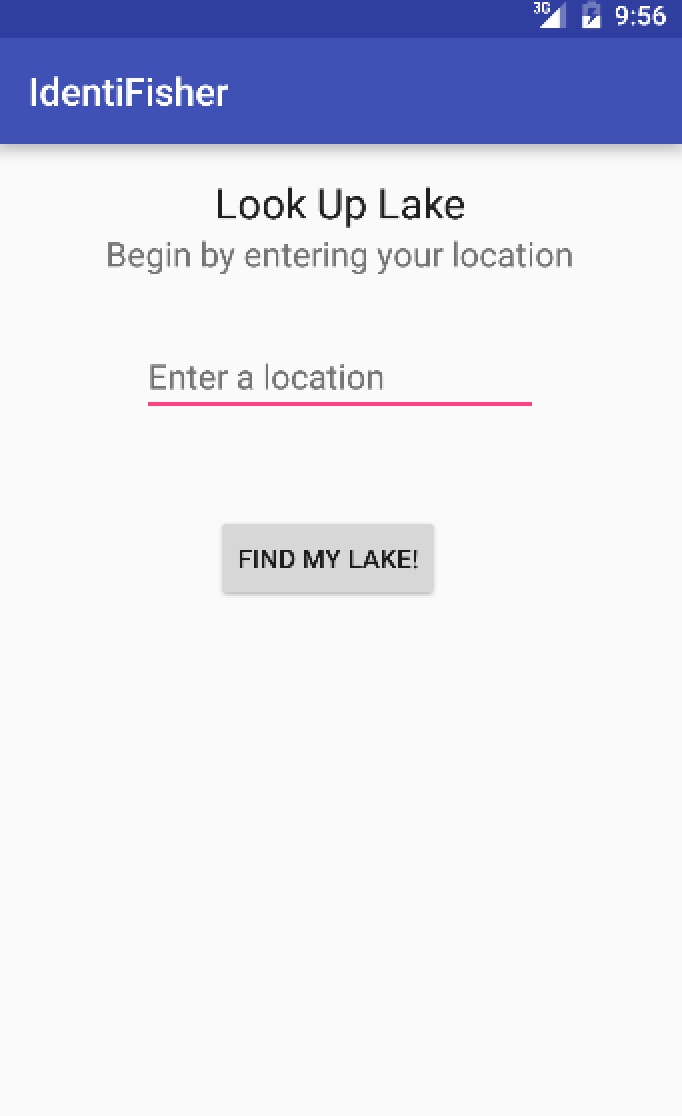
\includegraphics[scale=0.30]{Lookup.png}
	\caption{LOOK UP LAKE page of IdentiFisher Application}
\end{figure}

\subsection{ADD A FISH page}
The top of the page displays the title of the page and a message to help user understand the function of this page. There is a textfield to input the
location of the fish found. Example displayed in the textfield: \textit{42 Wallaby Way, Sydney}. There is also a \textit{DETECT MY LOCATION} button
to use the current location of the device as input. There is a drop down list of fish to choose from and an \textit{ADD FISH} button.\\
\begin{figure}[H]
	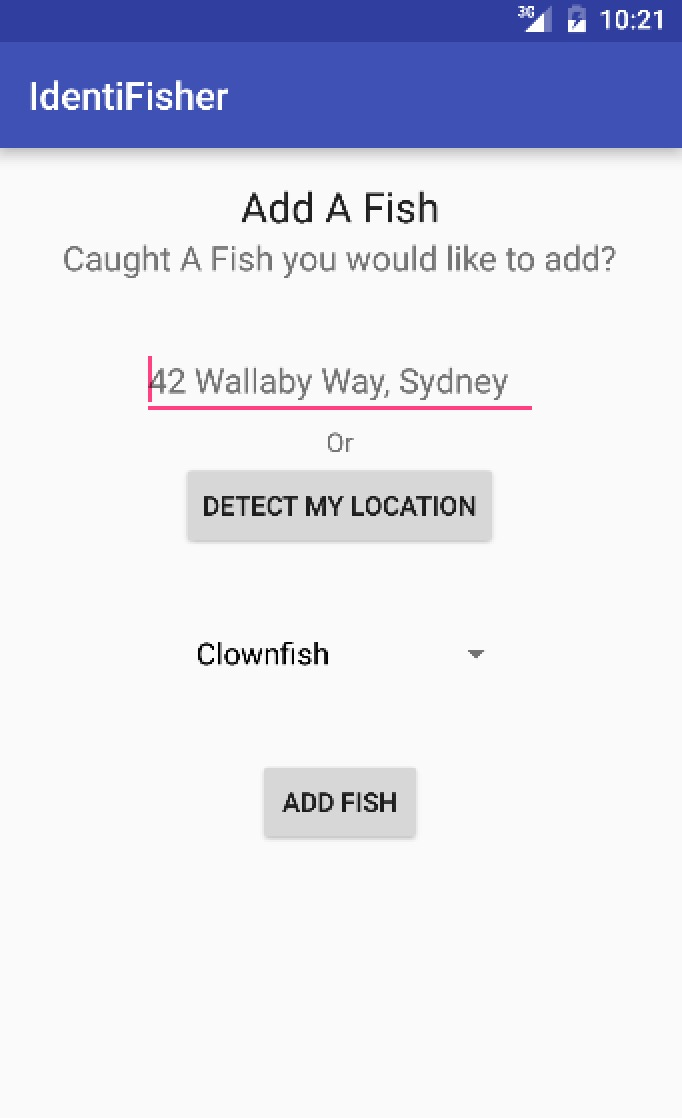
\includegraphics[scale=0.30]{AddFish.png}
	\caption{ADD A FISH page of IdentiFisher Application}
\end{figure}

\section{Examples}

\subsection{Identifying A Fish}
First open the application and click on \textit{IDENTIFISHER}. Begin by clicking on the drop down, and giving the best guess as to how to describe the fish you want to identify. After doing so, and being content with the properties, click on the Identify button. This will now try to identify the fish, and will list them from most likely to least likely in the drop down menu. Congratulations! You have offically identified a fish!

\subsection{Adding an Unknown Fish to the Database}
If you haven't identified the fish, go to the previous section to learn to do so. By now, the lower drop down menu should be populated. It is important to look at the most likely candidates, and choose the best one with your given knowledge. After deciding and clicking on said one, click Add Fish. Congratulations! You have offically identified a fish and added it to the database!

\section{Server Administrator Instructions}

\subsection{Swapping Experts}
In order to add an expert, follow these instructions
\begin{itemize} 
	\item Be Sure that the Expert being added is a child class to the Expert Class in the Application
	\item Increase the size of the Expert array by 1, as seen in the ExpertManager constructor
	\item Then fill new place in array with the new Expert child object, passing on any necessary information such as the encryption key
\end{itemize}
In order to delete an expert, follow these instructions
\begin{itemize} 
	\item Decrease the size of the Expert array by 1, as seen in the ExpertManager constructor
	\item Then delete the line where the array is filled with the Expert being deleted, and shift any current Experts if necessary 
\end{itemize}

\section{Functional Requirements}

\newpage
\listoffigures

\end{document}
